%!TEX root=paper.tex

\subsection{Utilization}
\label{sec:util}
 
  The default landing page of the dashboard presents an overview of all the endpoints, 
  which presents some basic utilization information as:
  (1) the number of calls to that endpoint since the begining of tracking
  (2) the number of calls in the last seven days, and
  (3) the number of calls in the last day


    \begin{figure}[h!]
      \centering
      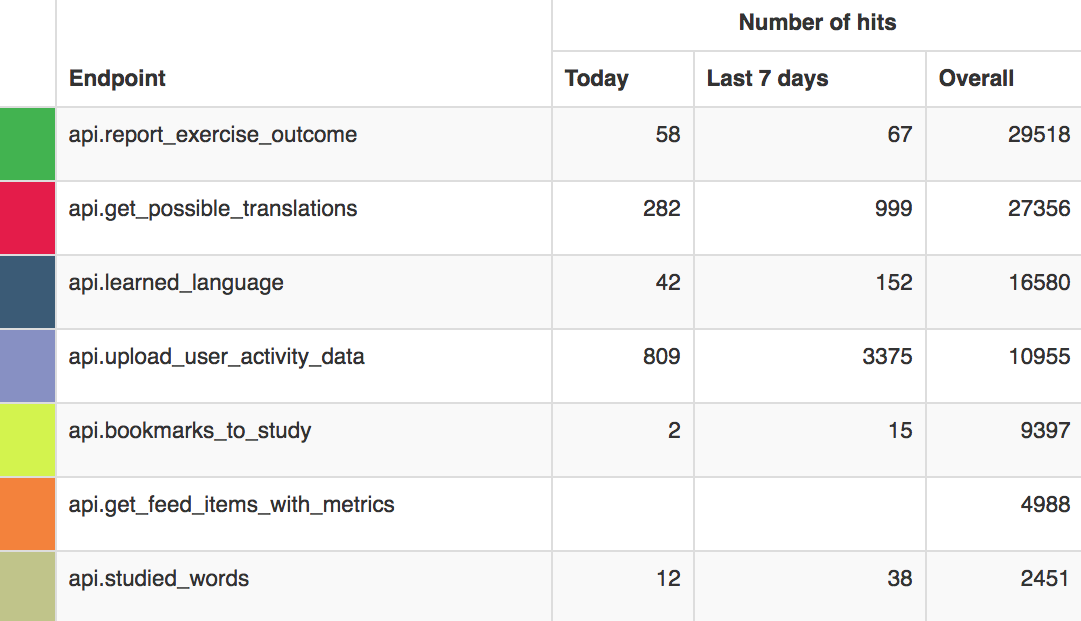
\includegraphics[width=0.8\linewidth]{utilization-table}
      \caption{The API Overview presents synthetic endpoint utilization information}
      \label{fig:basicest}
    \end{figure}

  This kind of information is already very useful, and can provide the API maintainer with insight into the evolution of their service API. The seven endpoints present in \Fref{fig:basicest} illustrate three types of insight that the maintainer can obtain by looking at such a view: 

  \begin{itemize}

    \item {\bf Service Specific Usage Patterns}. The two most used endpoints in the figure stand for the two main activities in the system: 

      \begin{itemize}

        \item \epTranslationsColor is an indicator of the amount of foreign language reading the users are doing. 

        \item \epOutcomeColor is an indicator of the amount of foreign vocabulary practice the users are doing.

      \end{itemize}

    \item {\bf Sudden Increase of Endpoint Usage}. One endpoint (\epUserActivityColor) has disproportionately been used in the last day and last week. 

    \item {\bf Possibly Discontinued Endpoint Usage}. One endpoint (\epFeedItemsColor) has not been used in the last 7 days. This might be an endpoint that is deprecated.

  \end{itemize}


\niceseparator


  For a more detailed view of utilization evolution, \Fref{fig:aeu} shows the \perspective{Daily API Utilization} perspective on API utilization that \tool provides: a stacked bar chart of the number of hits to various endpoints grouped by day\footnote{Endpoint colors are the same in different views}. \Fref{fig:aeu} in particular shows a peak utilization, on June 28, 2017 when the API had more than 12.000 hits\footnote{Turns out that the high school students that were using the system for their French-learning class had a deadline on that date}. 

    \begin{figure}[!ht]
    \centering
    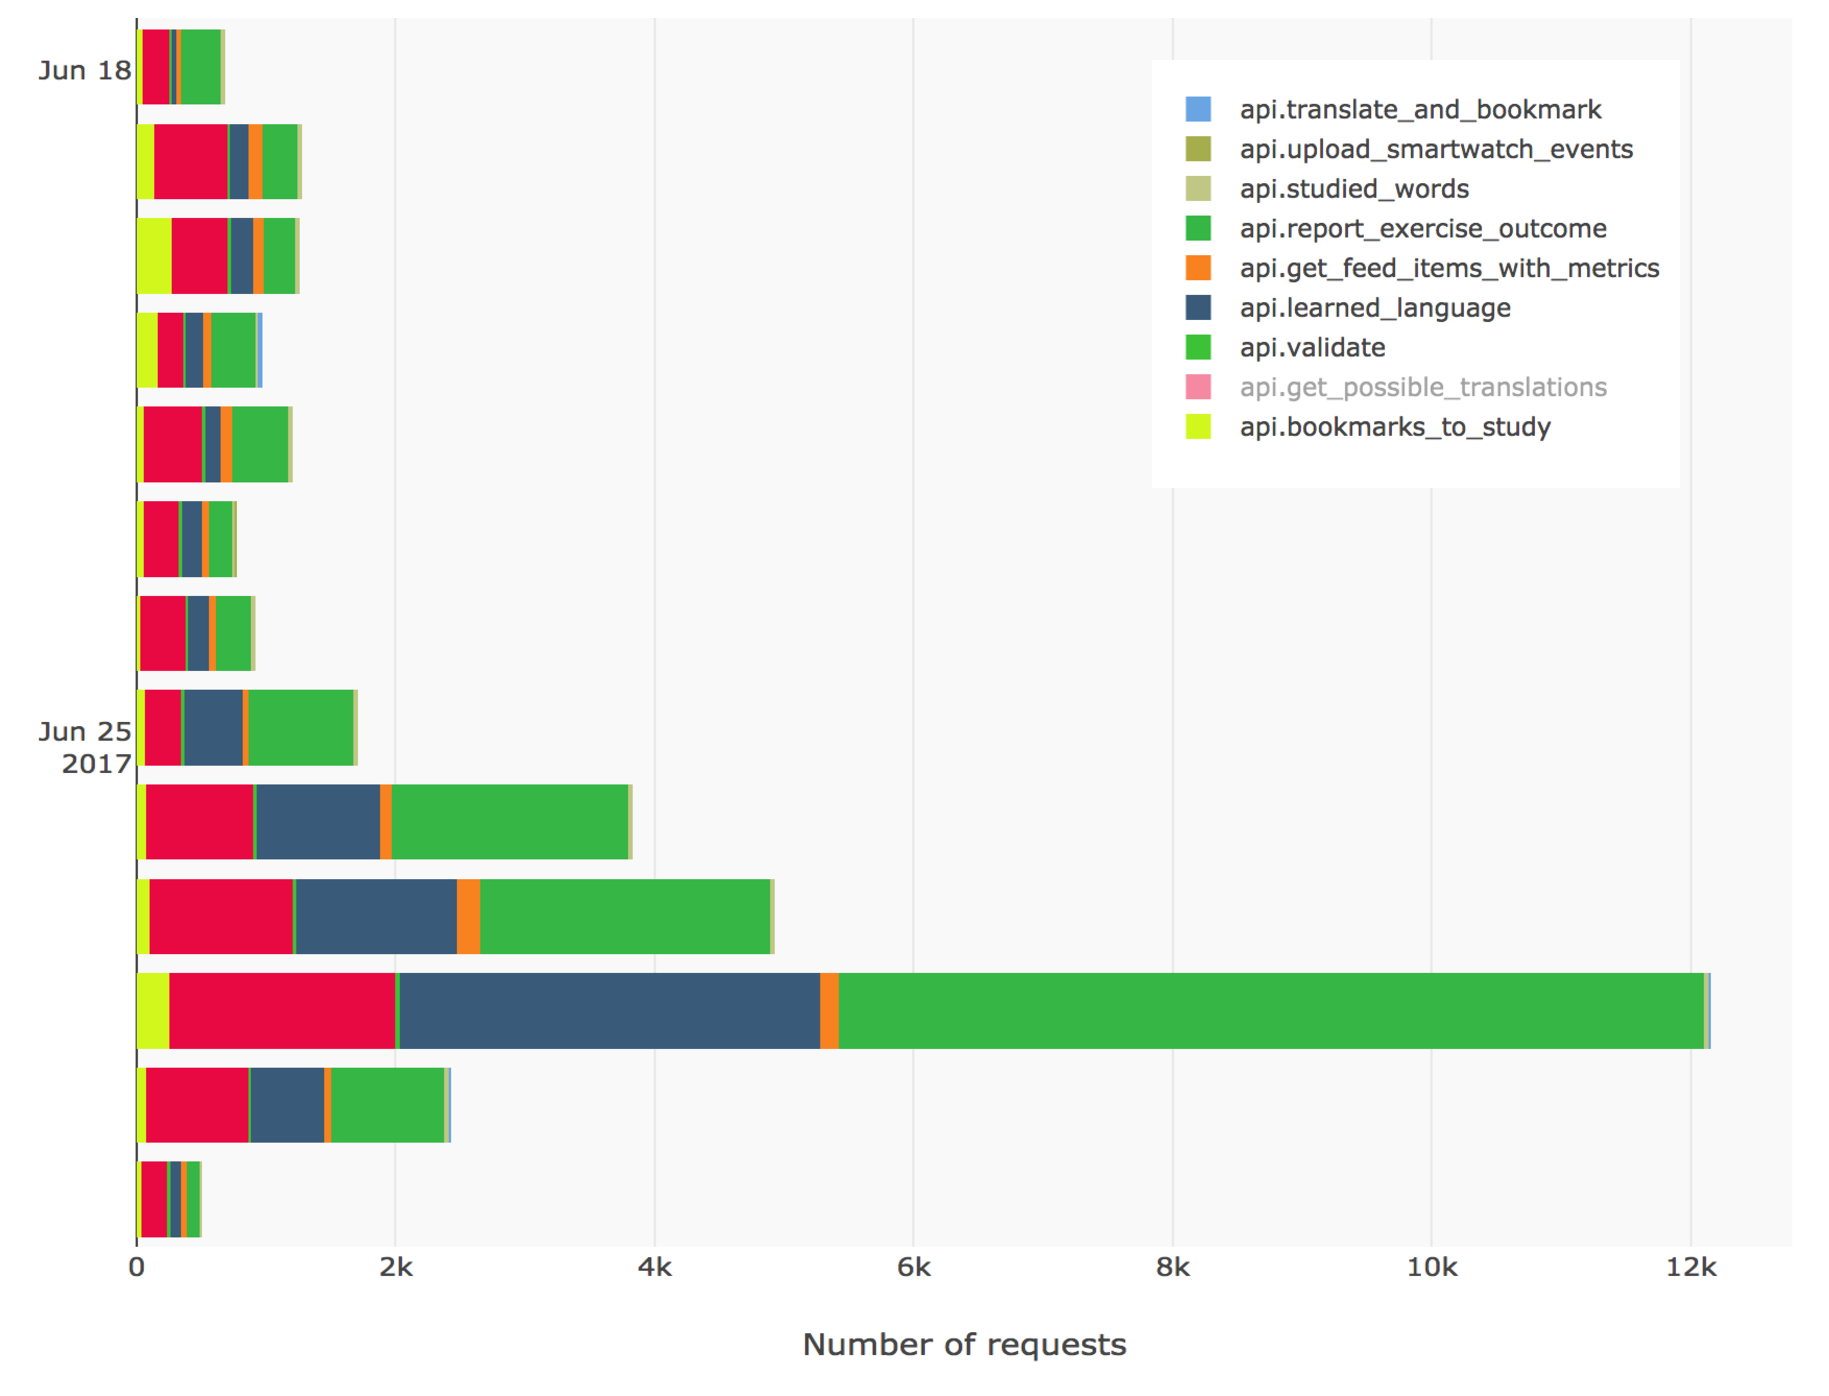
\includegraphics[width=0.8\linewidth]{number_of_requests_}
    \caption{Usage patterns become easy to spot in the requests per hour heatmap}
    \label{fig:aeu}
    \end{figure}


\niceseparator


  Another utilization perspective is the \perspective{Hourly API Utilization} in which  the \tool can highlight {\em cyclic patterns of usage per hour of day} by means of a heatmap, as in \Fref{fig:dp}. 


    \begin{figure}
      \centering
      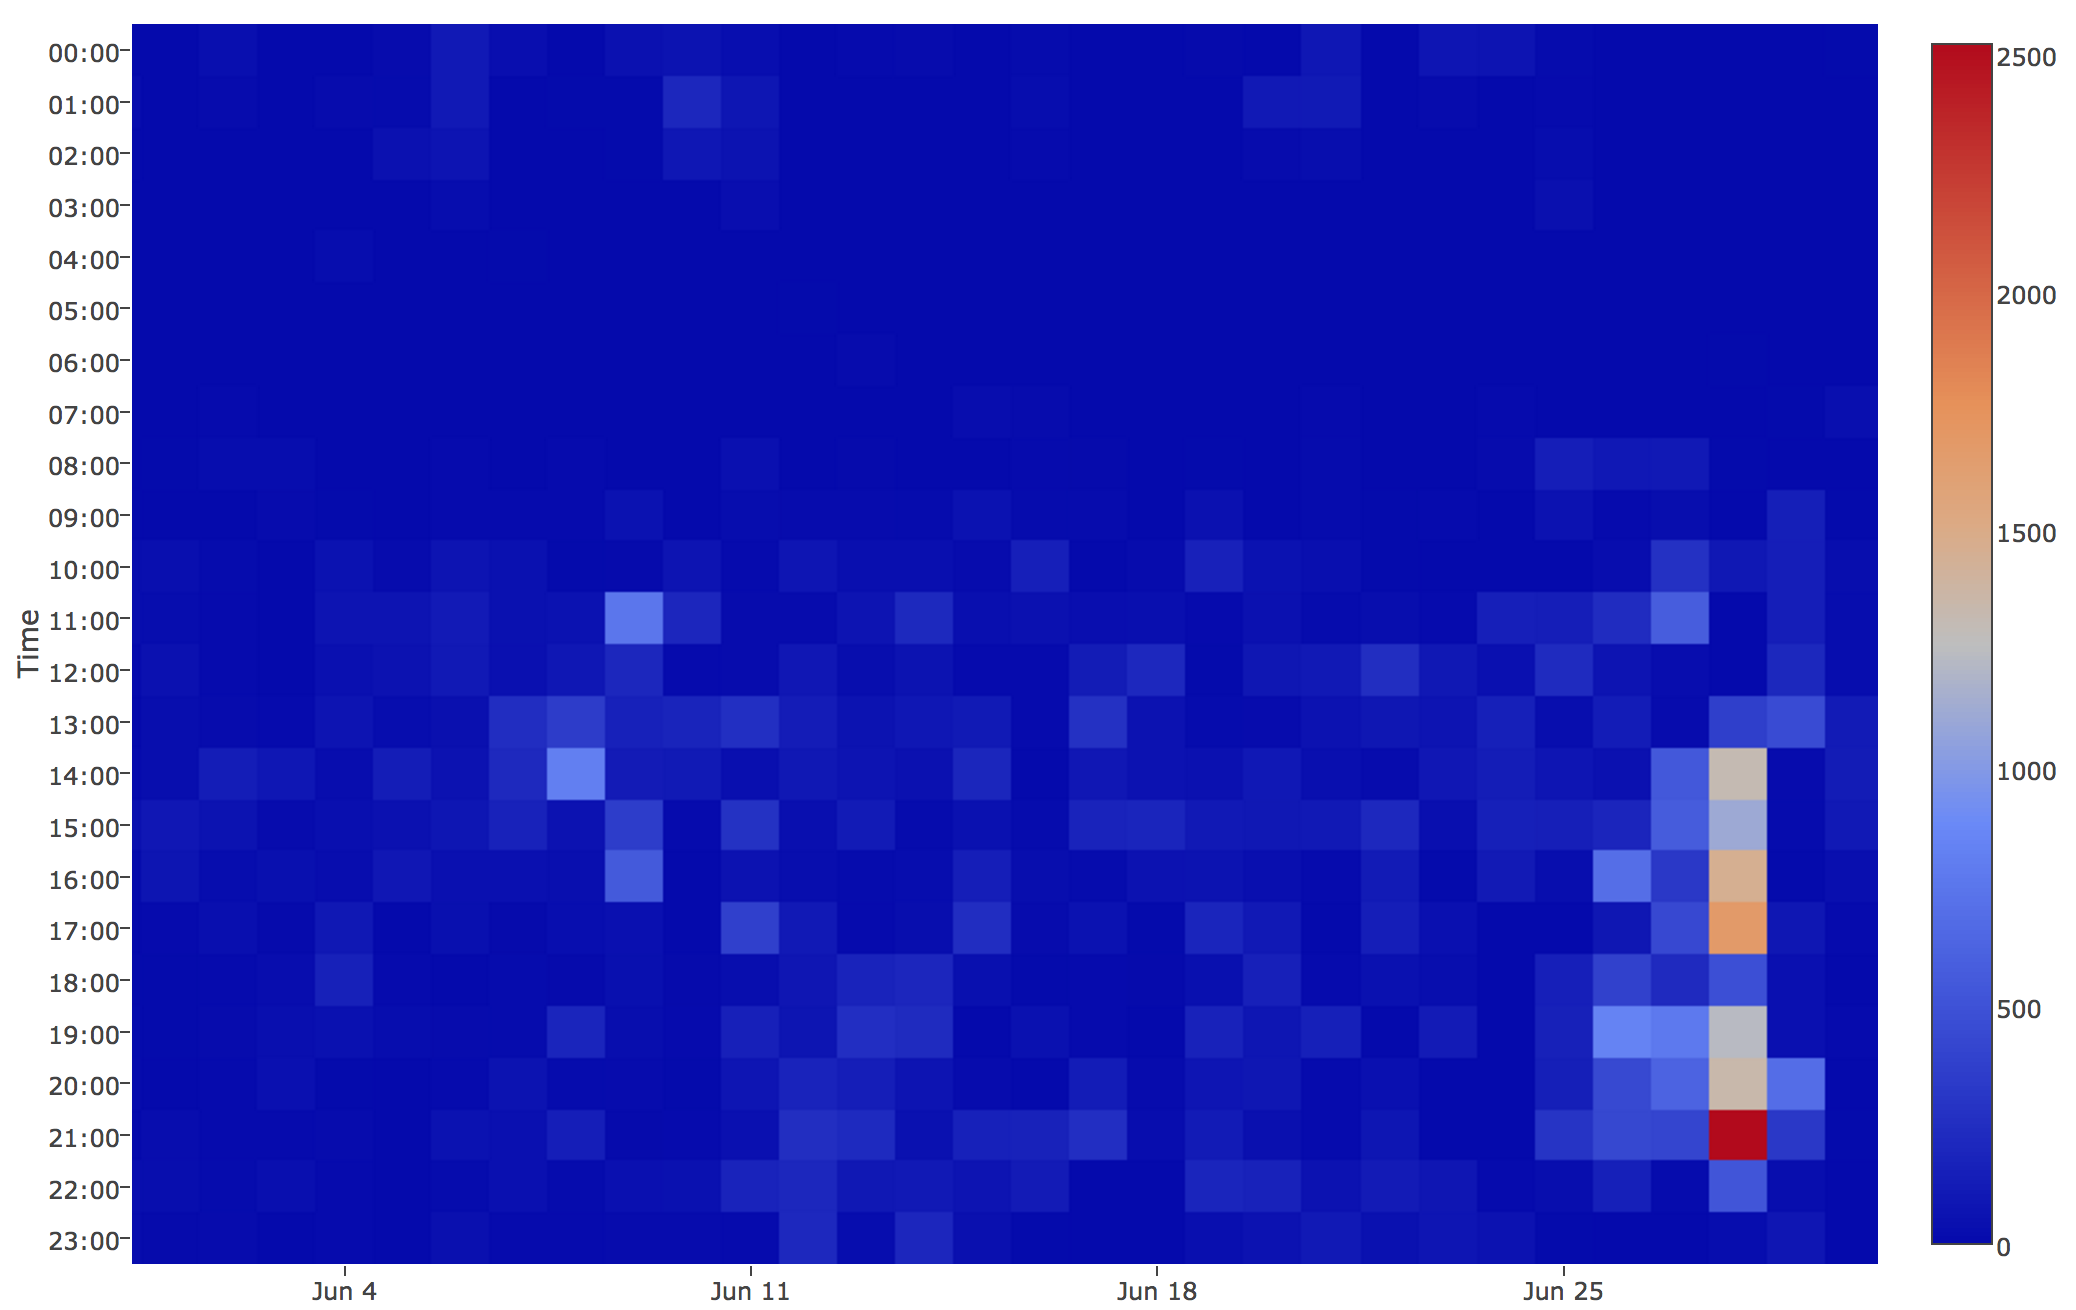
\includegraphics[width=0.8\linewidth]{daily_patterns_}
      \caption{Usage patterns become easy to spot in the requests per hour heatmap}
      \label{fig:dp}
    \end{figure}


  Figure \ref{fig:dp} shows the API not being used during the early morning hours, with most of the activity focused around working hours and some light activity during the evening. This is consistent with the fact that the current users are all in the central European timezone. Also, the figure shows that the spike in utilization that was visible also in the previous graph happended in on afternoon/evening.






